%!TeX encoding=UTF-8
%!TeX root=main.tex
%!TeX program=xelatex

\documentclass[aspectratio=169]{beamer}

\usetheme[sectionpage=progressbar,subsectionpage=progressbar,numbering=fraction,
          progressbar=foot]{metropolis}

\graphicspath{{../img/}}
\usepackage{svg}
\svgpath{{../img/}}

\usepackage{appendixnumberbeamer}

\usepackage{hyperref}

\usepackage{datetime}
\newdate{talkdate}{08}{03}{2018}

\usepackage[cache=false]{minted}
\usepackage{inconsolata}
\setmonofont{Inconsolata}
\newfontfamily\DejaSans{DejaVu Sans}

\usepackage{textcomp}

\usepackage{xpatch}
\usepackage[citestyle=authortitle,backend=bibtex]{biblatex}
\addbibresource{../bibl.bib}
\xapptobibmacro{cite}{\setunit{\nametitledelim}\printfield{year}}{}{}
\renewcommand{\footnotesize}{\scriptsize}

\title{Adaptating Amplified Unit Tests for Human Comprehension}

\date{\displaydate{talkdate} @ KTH}
\author{%
  Simon Bihel\hfill\href{mailto:simon.bihel@ens-rennes.fr}{\nolinkurl{simon.bihel@ens-rennes.fr}}\\
}
\institute{%
  University of Rennes I \\
  \'Ecole Normale Sup\'erieure de Rennes
}

\begin{document}

\maketitle

\begin{frame}{Mutation Testing}
  \begin{columns}
    \begin{column}{0.7\textwidth}
      \minipage[c][0.7\textheight][s]{\columnwidth}
      Evaluating the quality of a test suite by injecting bugs
      \vfill{}
      \visible<+(1)->{Examples of \emph{mutators}:
      \begin{itemize}
        \item change a \texttt{>} condition with \texttt{<};
        \item delete the body of a method.
      \end{itemize}}
      \vfill{}
      \metroset{block=fill}
      \begin{block}<+(1)->{Goal}
        Enhance test suite by detecting new mutants
      \end{block}
      \endminipage{}
    \end{column}
    \begin{column}{0.3\textwidth}
      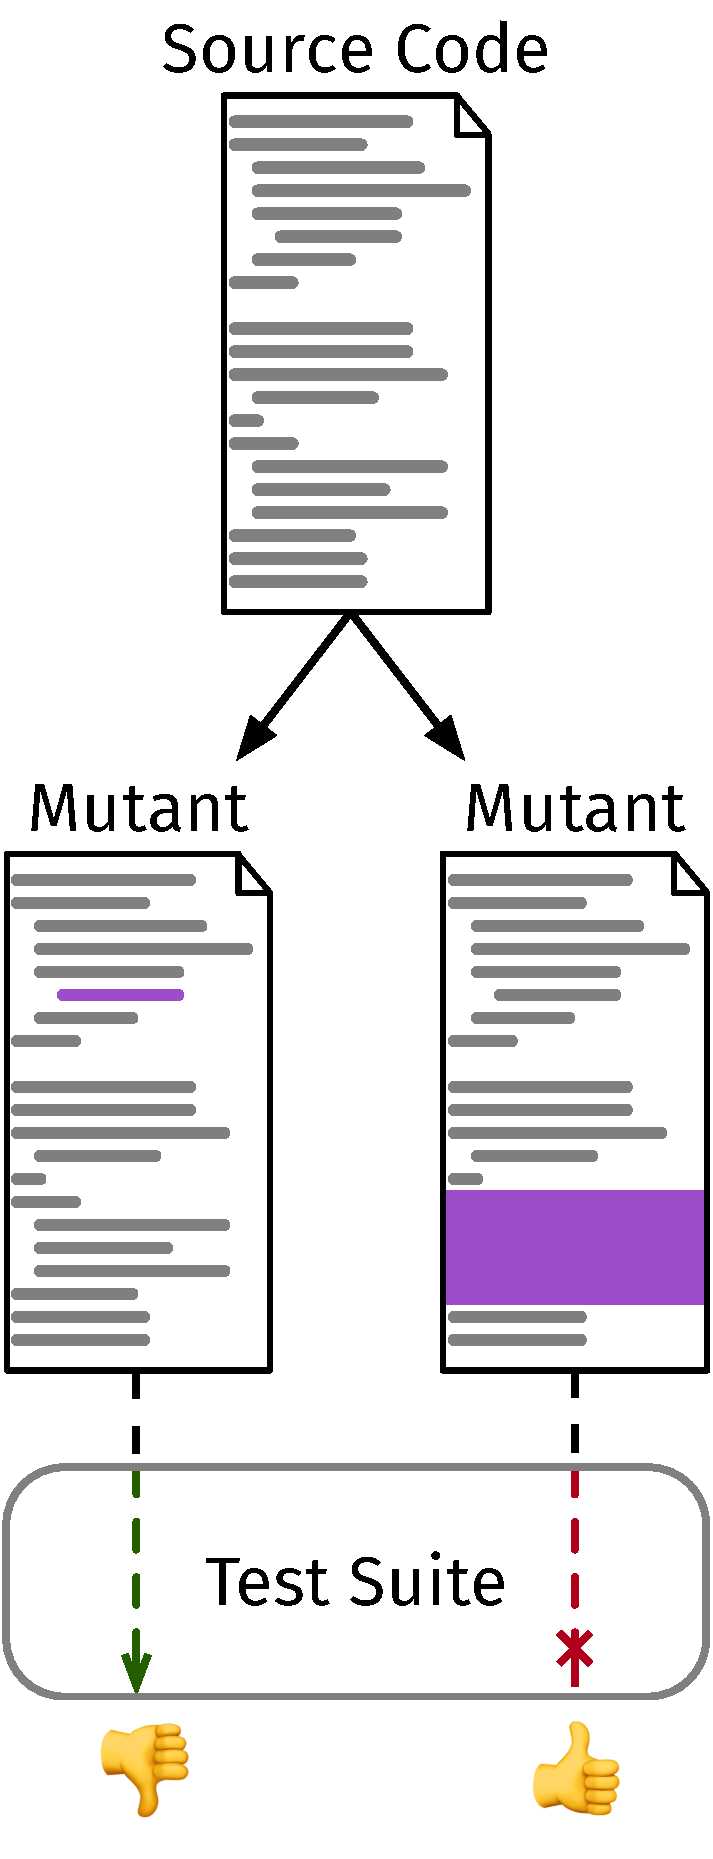
\includegraphics[height=\textheight]{mutation_testing}
    \end{column}
  \end{columns}
\end{frame}

\begin{frame}{DSpot\footnote{\url{https://github.com/STAMP-project/dspot}}}
  \begin{columns}
    \begin{column}{0.5\textwidth}
      Randomly modifies test cases:
      \begin{itemize}[<+(1)->]
        \item new inputs to trigger new behaviors;
        \item new assertions for unchecked properties;
        \item targets regression.
      \end{itemize}
    \end{column}
    \begin{column}{0.5\textwidth}
      \hspace*{-0.05\textwidth}
      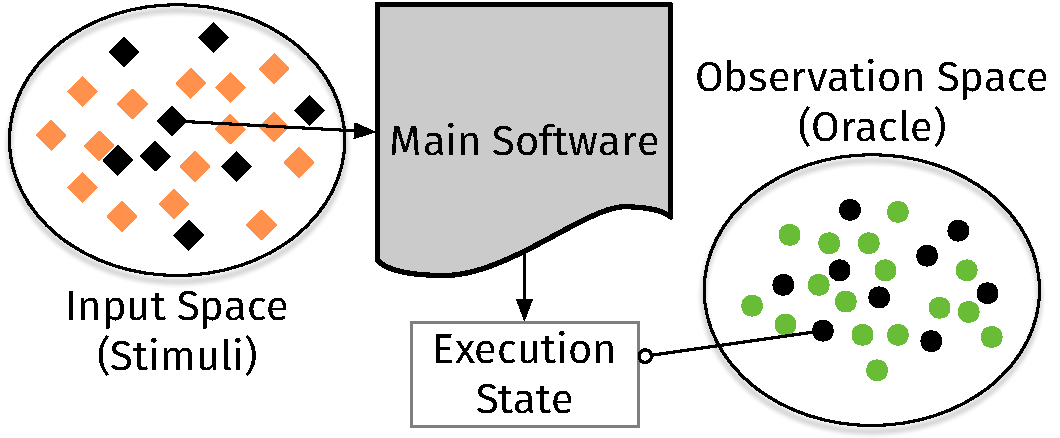
\includegraphics[width=1.1\textwidth]{spaces.pdf}
    \end{column}
  \end{columns}
  \vfill{}
  \visible<+(1)->{Benjamin Danglot, INRIA Lille, France}
\end{frame}

\begin{frame}[fragile]{Example\footnote{\href{https://github.com/google/guava/blob/ea66419b6aa52678816df77caa304e617255cca5/guava-tests/test/com/google/common/graph/ImmutableGraphTest.java\#L29-L40}{https://github.com/google/guava/blob/master/guava-tests/test/com/google/common/graph/ImmutableGraphTest.java\#L29-L40}}}
  \begin{minted}[linenos]{java}
@Test
public void immutableGraph() {
  MutableGraph<String> mutableGraph = GraphBuilder.directed().build();
  mutableGraph.addNode("A");
  ImmutableGraph<String> immutableGraph = ImmutableGraph.copyOf(mutableGraph);

  assertThat(immutableGraph).isNotInstanceOf(MutableValueGraph.class);
  assertThat(immutableGraph).isEqualTo(mutableGraph);

  mutableGraph.addNode("B");
  assertThat(immutableGraph).isNotEqualTo(mutableGraph);
}
  \end{minted}
\end{frame}

\begin{frame}[fragile]{Example of Amplification}
  \begin{minted}[linenos,highlightlines={5,9}]{java}
@Test
public void immutableGraph() {
  MutableGraph<String> mutableGraph = GraphBuilder.directed().build();
  mutableGraph.addNode("A");
  mutableGraph.addNode("C");
  ImmutableGraph<String> immutableGraph = ImmutableGraph.copyOf(mutableGraph);

  assertThat(immutableGraph).isNotInstanceOf(MutableValueGraph.class);
  assertTrue(immutableGraph.nodes().contains("A"));
  assertThat(immutableGraph).isEqualTo(mutableGraph);

  mutableGraph.addNode("B");
  assertThat(immutableGraph).isNotEqualTo(mutableGraph);
}
  \end{minted}
\end{frame}

\begin{frame}{Goal}
  \large{\textbf{\textrightarrow{} Human-friendly, high-level, natural language description}}
  \pause{}

  First objective: an explanation per mutant kill.
\end{frame}

\begin{frame}{Identify Relevant Statements}
  Identify the killing assertion.
  \pause{}
  \metroset{block=fill}
  \begin{block}{Simple static slicing:}
    \begin{itemize}
      \item starting from the killing assertion;
      \item control-flow slicing and
      \item data-flow slicing.
    \end{itemize}
  \end{block}
  \vfill{}
  \metroset{block=transparent}
  \begin{block}<+(1)->{Java slicing tool}
    T.J. Watson Libraries for Analysis (WALA)\footnote<+->{\url{https://github.com/wala/WALA}} %\only<+->{\footnote{\url{https://github.com/wala/WALA}}}

    Established library with active development.
  \end{block}
\end{frame}

\begin{frame}{Cleaning the Amplifications}
  Minimisation phase \textrightarrow{} less explanation to generate.
  \begin{enumerate}[<+(1)->]
    \item Remove assertions that never fail.
    \item Remove statements not present in a slice.
    \item Remove statements with no impact. \textrightarrow{} long process
  \end{enumerate}
  \pause{}
  \metroset{block=fill}
  \begin{block}{Minimizing only amplifications}
    \begin{itemize}
      \item Less time consuming.
      \item Keep the original part intact \textrightarrow{} better for understanding.
    \end{itemize}
  \end{block}
\end{frame}

\begin{frame}{Related Works --- Software Artifact Summarisation --- Software Maintenance}
  \metroset{block=fill}
  \begin{block}{\textit{UnitTestScribe}\footcite{li2016automatically}\footnote{\url{https://github.com/boyangwm/UnitTestScribe}}}
    \begin{itemize}[<+(1)->]
      \item[{
\includegraphics[width=1em]{Fxemoji_u1F389}}] Empirical study and survey \textrightarrow{} need for automated documentation.
      \item Summarises actions in natural language (Software Word Usage Model, method stereotypes). %\footcite{hill2010integrating}\footcite{dragan2006reverse} [{
\includegraphics[width=1em]{Emoji_u1f44d}}]
    \end{itemize}
  \end{block}
  \vfill{}
  \pause{}
  \begin{block}{Code changes summarisation (i.e.\ commit message generation)}
    Focused on general source code (add feature, fix bug, \dots).
  \end{block}
\end{frame}

\begin{frame}{Related Works Limit}
  \begin{block}{Problem}
    No ``why'' information. Paraphrasing the code.
  \end{block}
  \pause{}
  \textbf{Reason for amplifications to exist \textrightarrow{} mutant kill.}
\end{frame}

\begin{frame}{Natural Description}
  \metroset{block=fill}
  \begin{block}{Better oracle:}
    \begin{itemize}
      \item what part of the system was left out;
      \item avoid using terms as mutant.
    \end{itemize}
  \end{block}
  \pause{}
  \begin{block}{New kind of behaviour:}
    \begin{itemize}
      \item differences in traces to explain how a bug is triggered;
      \item use mutators stereotypes to explain how the inputs are modified.
    \end{itemize}
  \end{block}
\end{frame}

\begin{frame}{Experiment Protocol}
  \begin{itemize}[<+->]
    \item Study repos with strong commit message guidelines (e.g.\ Google).
    \item Performances.
    \item Survey with real developers.
  \end{itemize}
\end{frame}

\end{document}
